\documentclass[11pt]{article}

\usepackage[margin=2.5cm]{geometry}
\usepackage{amsmath,amssymb}
\usepackage{booktabs}
\usepackage{xcolor}
\usepackage[skins,breakable]{tcolorbox}
\usepackage{hyperref}
\usepackage{caption}
\usepackage{enumitem}
\usepackage{fancyhdr}
\usepackage{titlesec}

\usepackage{graphicx}
\graphicspath{{./images/}{./figs/}}


\definecolor{navy}{RGB}{20,40,90}
\definecolor{lgray}{RGB}{245,245,245}

\titleformat{\section}{\large\bfseries\color{navy}}{\thesection}{1em}{}
\titleformat{\subsection}{\normalsize\bfseries\color{navy}}{\thesubsection}{1em}{}

\pagestyle{fancy}
\fancyhf{}
\rhead{\small Narrative decomposition methodology}
\lhead{\small CNN Iran-War corpus}
\cfoot{\thepage}

\newtcolorbox{examplebox}[1]{
  colback=lgray, colframe=navy!60!black, fonttitle=\bfseries,
  title=#1, breakable, boxrule=0.6pt, arc=1mm
}

\title{\textbf{Clustering, Prototype Narratives, and Stiefel-Manifold\\
Orthogonalization: A Worked Methodology}\\[4pt]
\large Applied to a Corpus of CNN Live-Blog Coverage of the 2026 Iran War}
\author{Charles-Albert Lehalle,\\[.2em] following Anglade-Lehalle-Massi approach of orthogonalisation of narratives}
\date{Printed the Aug 21, 2026}

\begin{document}
\maketitle
\thispagestyle{fancy}

\begin{abstract}
\noindent This report documents the analytical pipeline applied to a corpus of
1{,}572 text snippets extracted from CNN's live-blog coverage of the
US--Israel--Iran conflict (March--August 2026). The pipeline (i) embeds and
clusters the snippets, in their \emph{natural, unmodified embedding space},
into eight thematic groups; (ii) for each cluster, defines a small set of
\emph{representative narratives} (short illustrative sentences) and averages
them into a single, more stable \emph{prototype of narrative}; (iii) removes
the mutual overlap between the eight prototypes by solving an optimization
problem on the Stiefel manifold, yielding what we call \emph{pure
narratives} --- versions of each prototype purged of the ``background
noise'' shared by all clusters (ordinary English grammar and the generic
vocabulary of Iran-war reporting); and (iv) scores every snippet against
the raw and pure prototypes to measure how well each representation
discriminates between themes. Because the pure narratives no longer carry
that shared background component, variation in a document's cosine
similarity to a pure narrative over time reflects variation in its
\emph{relative exposure to that specific narrative}, rather than drift in
generic war-reporting language. The central empirical result is that the
pure (orthogonalized) prototypes separate in-cluster from out-of-cluster
documents markedly better than the raw prototypes, which serves as an
\emph{ex post}, label-free validation of both the clustering and the
orthogonalization procedure. All steps are illustrated in detail on a
single cluster, \textit{Maritime Conflict \& Strait of Hormuz}.
\end{abstract}

% =========================================================================
\section{Overview of the pipeline}
% =========================================================================

The analysis proceeds in five stages, detailed in the sections that follow:

\begin{enumerate}[label=\textbf{Stage \arabic*.}, leftmargin=2.2cm]
    \item \textbf{Embed and cluster the corpus in its natural space.} Every paragraph-level snippet is embedded with a sentence-transformer and grouped into $K=8$ clusters using K-Means directly on this embedding space (after a variance-preserving PCA reduction, purely for numerical stability). \emph{No orthogonalization or other transformation is applied at this stage}: the clustering reflects the raw geometry of the embedding model.
    \item \textbf{Define representative narratives and average them into a prototype.} For each cluster, the analyst curates a small number of short, illustrative sentences (here, three, generated with the help of Gemini) called \emph{representative narratives}. Because a single representative narrative can be idiosyncratically worded, the three are embedded and \emph{averaged} (then re-normalized) into one more stable vector per cluster, the \emph{prototype of narrative}.
    \item \textbf{Orthogonalize the prototypes into ``pure'' narratives.} The eight prototype embeddings are projected onto an orthonormal basis via a custom \texttt{stiefel\_optimize} routine. The result is called a \emph{pure narrative}: a version of the prototype from which the ``background noise'' common to \emph{all} clusters --- generic English sentence structure and the shared vocabulary of Iran-war reporting --- has been removed, leaving (approximately) only what is specific to that one theme.
    \item \textbf{Score every document under three representations.} Each of the 1{,}572 snippets is compared (cosine similarity) against the \emph{original} prototypes, the \emph{pure (orthogonal)} prototypes, and the \emph{residual} (original $-$ pure) component --- the part of each prototype made up of exactly the shared background noise removed in Stage~3.
    \item \textbf{Validate ex post.} The separation between in-cluster and out-of-cluster similarity is compared across the three representations. Sharper separation under the pure-narrative representation is taken as evidence that the clustering captures real, distinguishable narrative axes, and that changes in similarity to a pure narrative over time reflect genuine shifts in a document's exposure to that narrative rather than shared background drift.
\end{enumerate}

% =========================================================================
\section{Stage 1: Embedding and clustering the corpus}
% =========================================================================

The raw corpus consists of daily CNN live-blog pages, each split into
paragraph-level snippets after removing boilerplate (navigation text,
``Get our five biggest...'', duplicated live-coverage banners, etc.), leaving
$n = 1{,}572$ snippets spanning March 1 -- August 18, 2026.

\subsection{Embedding}
Each snippet $s_i$ is mapped to a unit-norm vector
$\mathbf{e}_i \in \mathbb{R}^{768}$ using a sentence-embedding model
(\texttt{nomic-ai/modernbert-embed-base}), so that cosine similarity between
two snippets reduces to a simple dot product:
\[
\text{sim}(s_i, s_j) = \frac{\mathbf{e}_i^\top \mathbf{e}_j}{\lVert \mathbf{e}_i\rVert\,\lVert \mathbf{e}_j\rVert} = \mathbf{e}_i^\top \mathbf{e}_j \quad (\text{since } \lVert \mathbf{e}_i\rVert = 1).
\]

\subsection{Dimensionality reduction and clustering}
\textbf{Important methodological point:} clustering is performed entirely in
the \emph{natural embedding space} of the snippets, i.e.\ on the raw
sentence-transformer output (after the linear, variance-preserving PCA step
described below). No orthogonalization, background-noise removal, or any
other transformation from later stages is applied before or during
clustering. This matters for the validity of Stage~5: whatever structure
K-Means finds is a property of the embedding model and the corpus alone,
not an artifact of the orthogonalization machinery introduced afterwards.

Because K-Means and Euclidean distances behave poorly in very
high-dimensional, near-uniform embedding spaces, the 768-dimensional
embeddings are first projected to 50 dimensions with PCA. K-Means with
$K=8$ clusters is then fit on the PCA scores (\emph{not} on the 2D t-SNE
coordinates, which are used only for visualization and would distort
distances). Each resulting cluster is inspected manually and given a
short thematic label. Table~\ref{tab:clusters} lists the eight clusters
and their size; full descriptions, rationale, and illustrative excerpts
for every cluster are given in Appendix~\ref{app:clusters}. The cluster
used as a worked example throughout the main text is
\textit{Maritime Conflict \& Strait of Hormuz} ($n=215$), which groups
reporting on shipping disruption, tanker attacks, naval blockades, and
transit through the Strait of Hormuz.

\begin{table}[htbp]
\centering
\caption{The eight K-Means clusters, their thematic label, and the number
of text snippets assigned to each ($n=1{,}572$ total). Full descriptions
are given in Appendix~\ref{app:clusters}.}
\label{tab:clusters}
\begin{tabular}{clr}
\toprule
\textbf{Cluster} & \textbf{Theme} & \textbf{Size} \\
\midrule
0 & Gulf Regional Military Escalation                & 209 \\
1 & Global Energy Markets \& Economic Fallout         & 81  \\
2 & Iranian Political Transition \& Internal Affairs  & 110 \\
3 & US-Israel Military Campaign in Iran               & 246 \\
4 & US Domestic Politics \& Presidential Leadership   & 306 \\
5 & Israel-Hezbollah-Lebanon Theater                  & 170 \\
6 & Diplomacy \& International Mediation              & 235 \\
7 & Maritime Conflict \& Strait of Hormuz             & 215 \\
\midrule
  & \textbf{Total}                                    & \textbf{1{,}572} \\
\bottomrule
\end{tabular}
\end{table}

\begin{figure}[htbp]
\centering
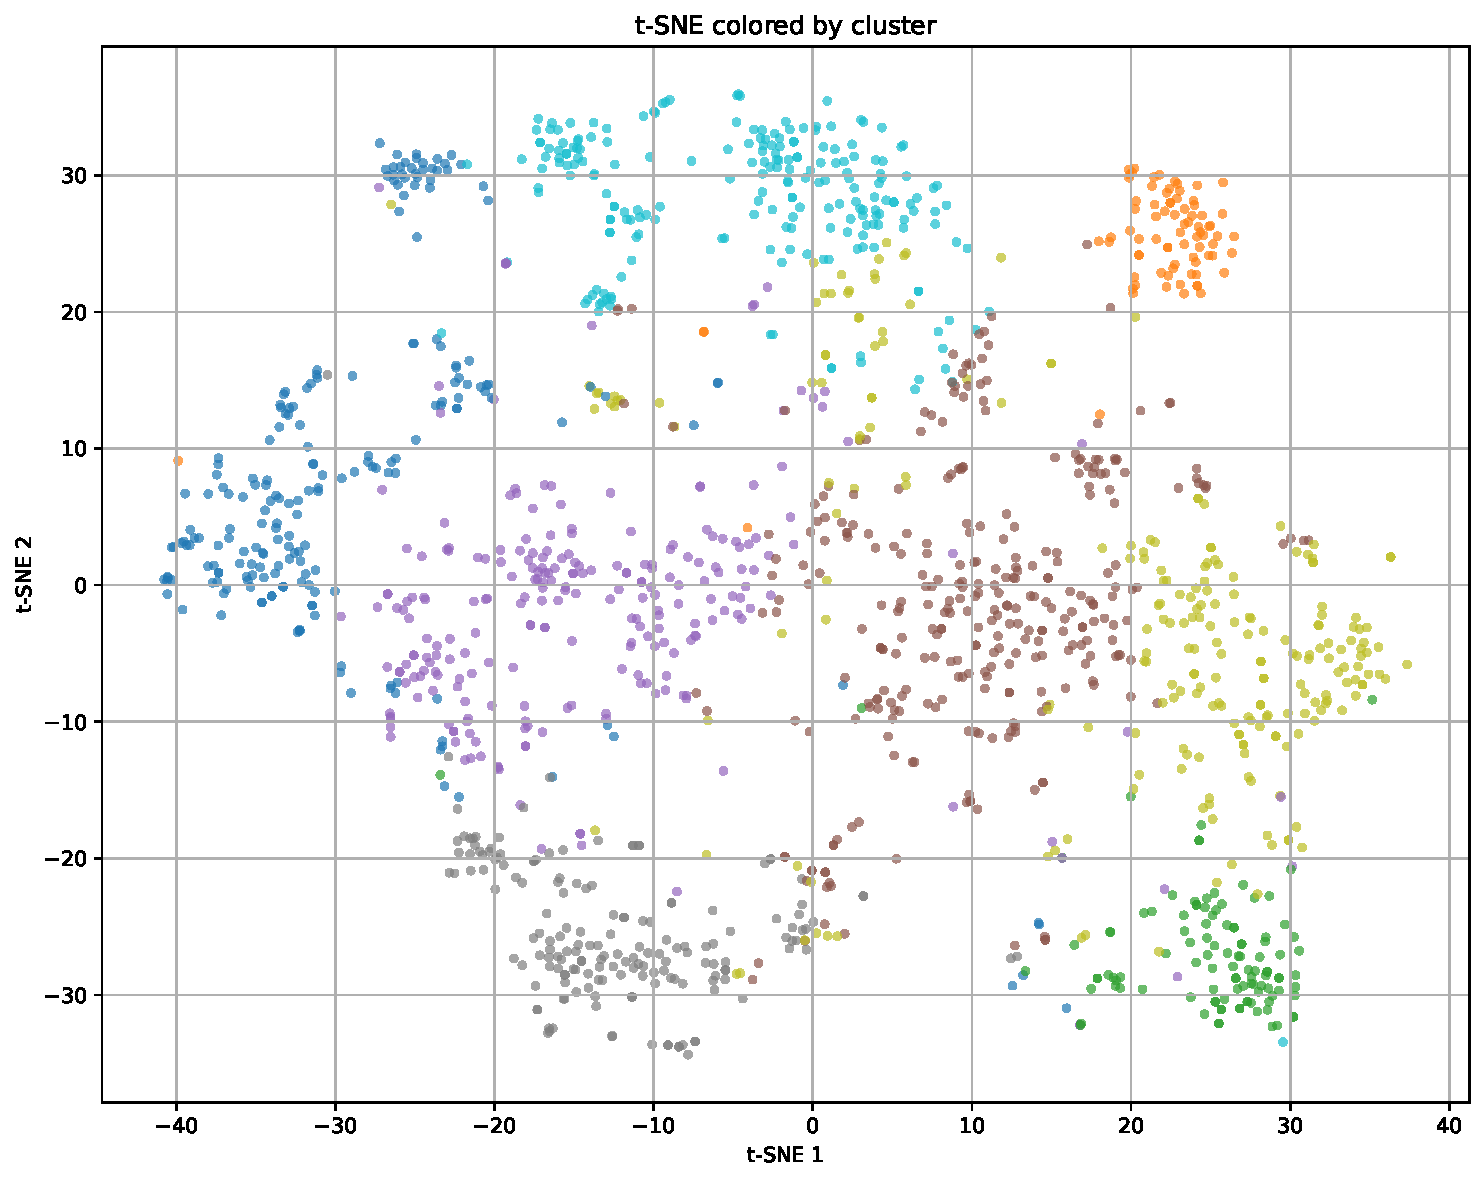
\includegraphics[width=0.92\textwidth]{clusters_CNN.pdf}
\caption{t-SNE projection (2 dimensions, computed on the same PCA-reduced,
natural embedding space used for K-Means, cosine metric, perplexity
$\approx 35$) of all 1{,}572 snippets, colored by their K-Means cluster
label. \textbf{This plot is diagnostic only}: t-SNE is used purely to
\emph{visualize} the clustering after the fact; K-Means itself, as stressed
above, is fit on the 50-dimensional PCA scores, never on these 2D
coordinates. Two qualitative features are worth noting. First, most
clusters form spatially coherent, largely non-overlapping blobs --- direct
visual confirmation that the eight themes correspond to genuinely separable
regions of the natural embedding space, consistent with the quantitative
separation reported in Section~\ref{sec:stage5}. Second, the larger clusters
(e.g.\ \textit{US Domestic Politics}, $n=306$, or \textit{US-Israel Military
Campaign}, $n=246$) tend to appear as elongated or multi-lobed regions
rather than single tight blobs, indicating that they are internally more
heterogeneous, likely covering several recurring sub-topics under one
broad label; smaller, more topically narrow clusters (e.g.\
\textit{Global Energy Markets}, $n=81$) instead form a single dense clump.
Scattered points sitting between two blobs are boundary snippets that
share vocabulary with more than one theme --- exactly the kind of shared
background noise that the Stiefel orthogonalization (Section~\ref{sec:stage3})
is designed to factor out when scoring documents against a narrative.}
\label{fig:tsne}
\end{figure}

% =========================================================================
\section{Stage 2: Representative narratives and the prototype of narrative}
% =========================================================================

\subsection{Representative narratives}
For each of the $K=8$ clusters, three short sentences are curated as
\emph{representative narratives}: text generated with the help of Gemini and
selected by the analyst to be illustrative of that theme. We denote the
three representative-narrative embeddings for cluster $i$ by
$\mathbf{r}_{i,1}, \mathbf{r}_{i,2}, \mathbf{r}_{i,3} \in \mathbb{R}^{768}$.
This choice is deliberately not automated (e.g., not the medoid or centroid
of the cluster): it encodes the analyst's semantic understanding of what the
theme \emph{is}, independently of how K-Means happened to partition the
data.

\begin{examplebox}{Worked example --- representative narratives for \textit{Maritime Conflict \& Strait of Hormuz}}
\begin{enumerate}[label=$\mathbf{r}_{7,\arabic*}$:, leftmargin=1.5cm]
\item Maritime traffic through the Strait of Hormuz has slowed to a near halt as shipping companies reroute or suspend passage.
\item US forces intercepted and seized a cargo vessel attempting to bypass the naval blockade of Iranian ports.
\item An oil tanker was struck and disabled by an unidentified projectile near the strait's entrance.
\end{enumerate}
\end{examplebox}

\subsection{From representative narratives to a prototype of narrative}
A single representative narrative can be idiosyncratically worded and is a
noisy estimate of ``what the theme is about'' in embedding space. To obtain
a more stable anchor, the three representative-narrative embeddings of each
cluster are \emph{averaged and re-normalized} into one vector, which we call
the \textbf{prototype of narrative} for that cluster:
\[
\mathbf{N}_i \;=\; \frac{\tfrac{1}{3}\sum_{k=1}^{3} \mathbf{r}_{i,k}}{\left\lVert \tfrac{1}{3}\sum_{k=1}^{3} \mathbf{r}_{i,k} \right\rVert}, \qquad i = 1,\dots,8,
\]
giving an $8\times 768$ matrix $\mathbf{N}$ of prototypes across all
clusters. It is this averaged prototype $\mathbf{N}_i$ --- not the
individual representative narratives $\mathbf{r}_{i,k}$ --- that is used as
the input to the orthogonalization step (Stage~3) and to all downstream
scoring (Stage~4). Averaging three phrasings of the same idea cancels out
some of each individual sentence's idiosyncratic wording while keeping the
direction that is common to all three, which is precisely the theme itself.

% =========================================================================
\section{Stage 3: Orthogonalization on the Stiefel manifold}
\label{sec:stage3}
% =========================================================================

\subsection{Motivation: separating signal from shared background noise}
Figure~\ref{fig:heatmap} (top-left $8\times8$ block) shows the pairwise
cosine similarity between the eight prototypes of narrative $\mathbf{N}_i$
built in Stage~2. Off-diagonal values of $0.6$--$0.8$ are common: prototypes
for genuinely distinct themes still point in very similar directions. We
interpret this shared component as a \textbf{common background noise} made
of two ingredients that every English sentence about this conflict carries,
almost regardless of its specific theme: (a) ordinary \emph{English
grammar and sentence structure} (subject-verb-object patterns, connective
words, tense markers), and (b) the \emph{generic vocabulary of Iran-war
reporting} shared across all eight themes (place names, military and
diplomatic jargon, recurring proper nouns such as ``Iran'', ``Trump'',
``strikes''). Because this background noise is present in \emph{every}
prototype, it is exactly the part of $\mathbf{N}_i$ that is problematic for
discrimination: a snippet can score highly against several prototypes
simultaneously merely because the prototypes themselves share this
background noise, not because the snippet is thematically ambiguous. The
goal of orthogonalization is to strip this shared component out and isolate
what we call the \textbf{pure narrative} of each theme.

\subsection{The optimization problem}
The goal is to find, for each prototype $\mathbf{N}_i$, a new vector
$\mathbf{V}_i$ such that:
\begin{itemize}
    \item the set $\{\mathbf{V}_i\}$ is \emph{exactly orthonormal}: $\mathbf{V}\mathbf{V}^\top = I$, i.e.\ $\mathbf{V}$ lies on the \textbf{Stiefel manifold} $\mathrm{St}(K, d) = \{V \in \mathbb{R}^{K\times d} : VV^\top = I_K\}$;
    \item each $\mathbf{V}_i$ remains \emph{as close as possible} to its original direction $\mathbf{N}_i$, so that the orthogonalized narrative is still recognizably about the same theme.
\end{itemize}

Formally, writing $\langle \mathbf{N}_i, \mathbf{V}_i\rangle$ for the
alignment (cosine similarity) between the $i$-th original and orthogonalized
prototype, the routine \texttt{stiefel\_optimize} solves
\[
\max_{V \in \mathrm{St}(K,d)} \; \min_{i=1,\dots,K} \; \langle \mathbf{N}_i, \mathbf{V}_i \rangle ,
\]
i.e.\ it maximizes the \emph{worst-case} alignment across all $K$ prototypes,
so that no single narrative is sacrificed to improve the others. Because the
hard $\min$ is non-smooth, the implementation uses a smooth \emph{soft-min}
surrogate with temperature $\tau$ (here $\tau=0.05$):
\[
\text{softmin}_\tau(x_1,\dots,x_K) = -\tau \log \sum_{i=1}^K \exp\!\left(-\frac{x_i}{\tau}\right), \qquad x_i = \langle \mathbf{N}_i, \mathbf{V}_i\rangle,
\]
which is minimized (cost $= -\text{softmin}$) using Riemannian conjugate
gradient descent (\texttt{pymanopt}'s \texttt{ConjugateGradient} optimizer),
initialized from a Gram--Schmidt orthogonalization of $\mathbf{N}$. Convergence
is fast: 24--40 iterations, a few seconds of wall-clock time.

\subsection{Interpretation of the three vectors}
\label{sec:interpretation}
For every cluster $i$, the procedure yields three related, comparable objects:
\begin{itemize}
    \item \textbf{Prototype (original)} $\mathbf{N}_i$: the averaged, re-normalized representative-narrative embedding from Stage~2 --- contains both theme-specific signal \emph{and} the shared background noise (grammar + generic war vocabulary).
    \item \textbf{Pure narrative (orthogonal)} $\mathbf{V}_i$: the Stiefel-projected version, mutually orthogonal to all other $\mathbf{V}_j$ ($j \ne i$) by construction --- our approximation of the narrative's content \emph{net of the shared background noise}, i.e.\ what is genuinely unique to theme $i$.
    \item \textbf{Residual (background noise)} $\mathbf{R}_i = \dfrac{\mathbf{N}_i - \mathbf{V}_i}{\lVert \mathbf{N}_i - \mathbf{V}_i \rVert}$: the (renormalized) component removed from the prototype to obtain the pure narrative --- our estimate of the shared grammar/vocabulary signal that theme $i$'s prototype has in common with the other themes.
\end{itemize}

\paragraph{Why this matters for interpreting cosine similarity.} Because the
pure narrative $\mathbf{V}_i$ is (by construction) purged of the background
noise common to all eight themes, a document's cosine similarity to
$\mathbf{V}_i$ is not inflated or deflated by how much generic
``war-reporting English'' that document happens to contain. Consequently,
when we later track $\mathbf{e}_t^\top \mathbf{V}_i$ over time or across
documents (Stage~4--5), movements in that quantity can be attributed to
genuine changes in the document's \emph{relative exposure to the pure
narrative $i$ itself}, rather than to incidental drift in how much generic
conflict vocabulary a given day's reporting happens to use. This is the
key property that the original, non-orthogonalized prototypes $\mathbf{N}_i$
do \emph{not} have: two documents could differ in $\mathbf{e}_t^\top
\mathbf{N}_i$ simply because one is written in a more ``typical war-report''
style, with no difference in actual exposure to theme $i$.

\begin{examplebox}{Worked example --- from prototype to pure narrative for \textit{Maritime Conflict}}
The prototype $\mathbf{N}_{\text{Maritime}}$ has cosine similarity
$\approx 0.78$ with $\mathbf{N}_{\text{US-Israel Military Campaign}}$ and
$\approx 0.71$ with $\mathbf{N}_{\text{Diplomacy}}$ (see
Fig.~\ref{fig:heatmap}, row \textit{Maritime Conflict \& Strait of Hormuz},
top-left block): both share heavy ``military operations'' and
``negotiation'' vocabulary --- exactly the kind of background noise
described above. After optimization, the pure narrative
$\mathbf{V}_{\text{Maritime}}$ has, by construction, cosine similarity
$\approx 0.00$ with every other pure narrative $\mathbf{V}_j$
(Fig.~\ref{fig:heatmap}, ``orth'' block, off-diagonal entries), while
retaining an alignment of $0.77$ with its own prototype direction
$\mathbf{N}_{\text{Maritime}}$ (diagonal of the original$\times$orth
block): the pure narrative is still recognizably ``about'' maritime
conflict, just stripped of what it shared with the rest of the corpus. The
corresponding residual (background-noise estimate)
$\mathbf{R}_{\text{Maritime}}$ instead correlates strongly
\emph{positively} with the other clusters' prototypes (0.51--0.67,
bottom-left block of Fig.~\ref{fig:heatmap}) and negatively with its own
pure narrative ($-0.48$), confirming that it isolates exactly the shared,
non-discriminative component that orthogonalization removed.
\end{examplebox}

\begin{figure}[htbp]
\centering
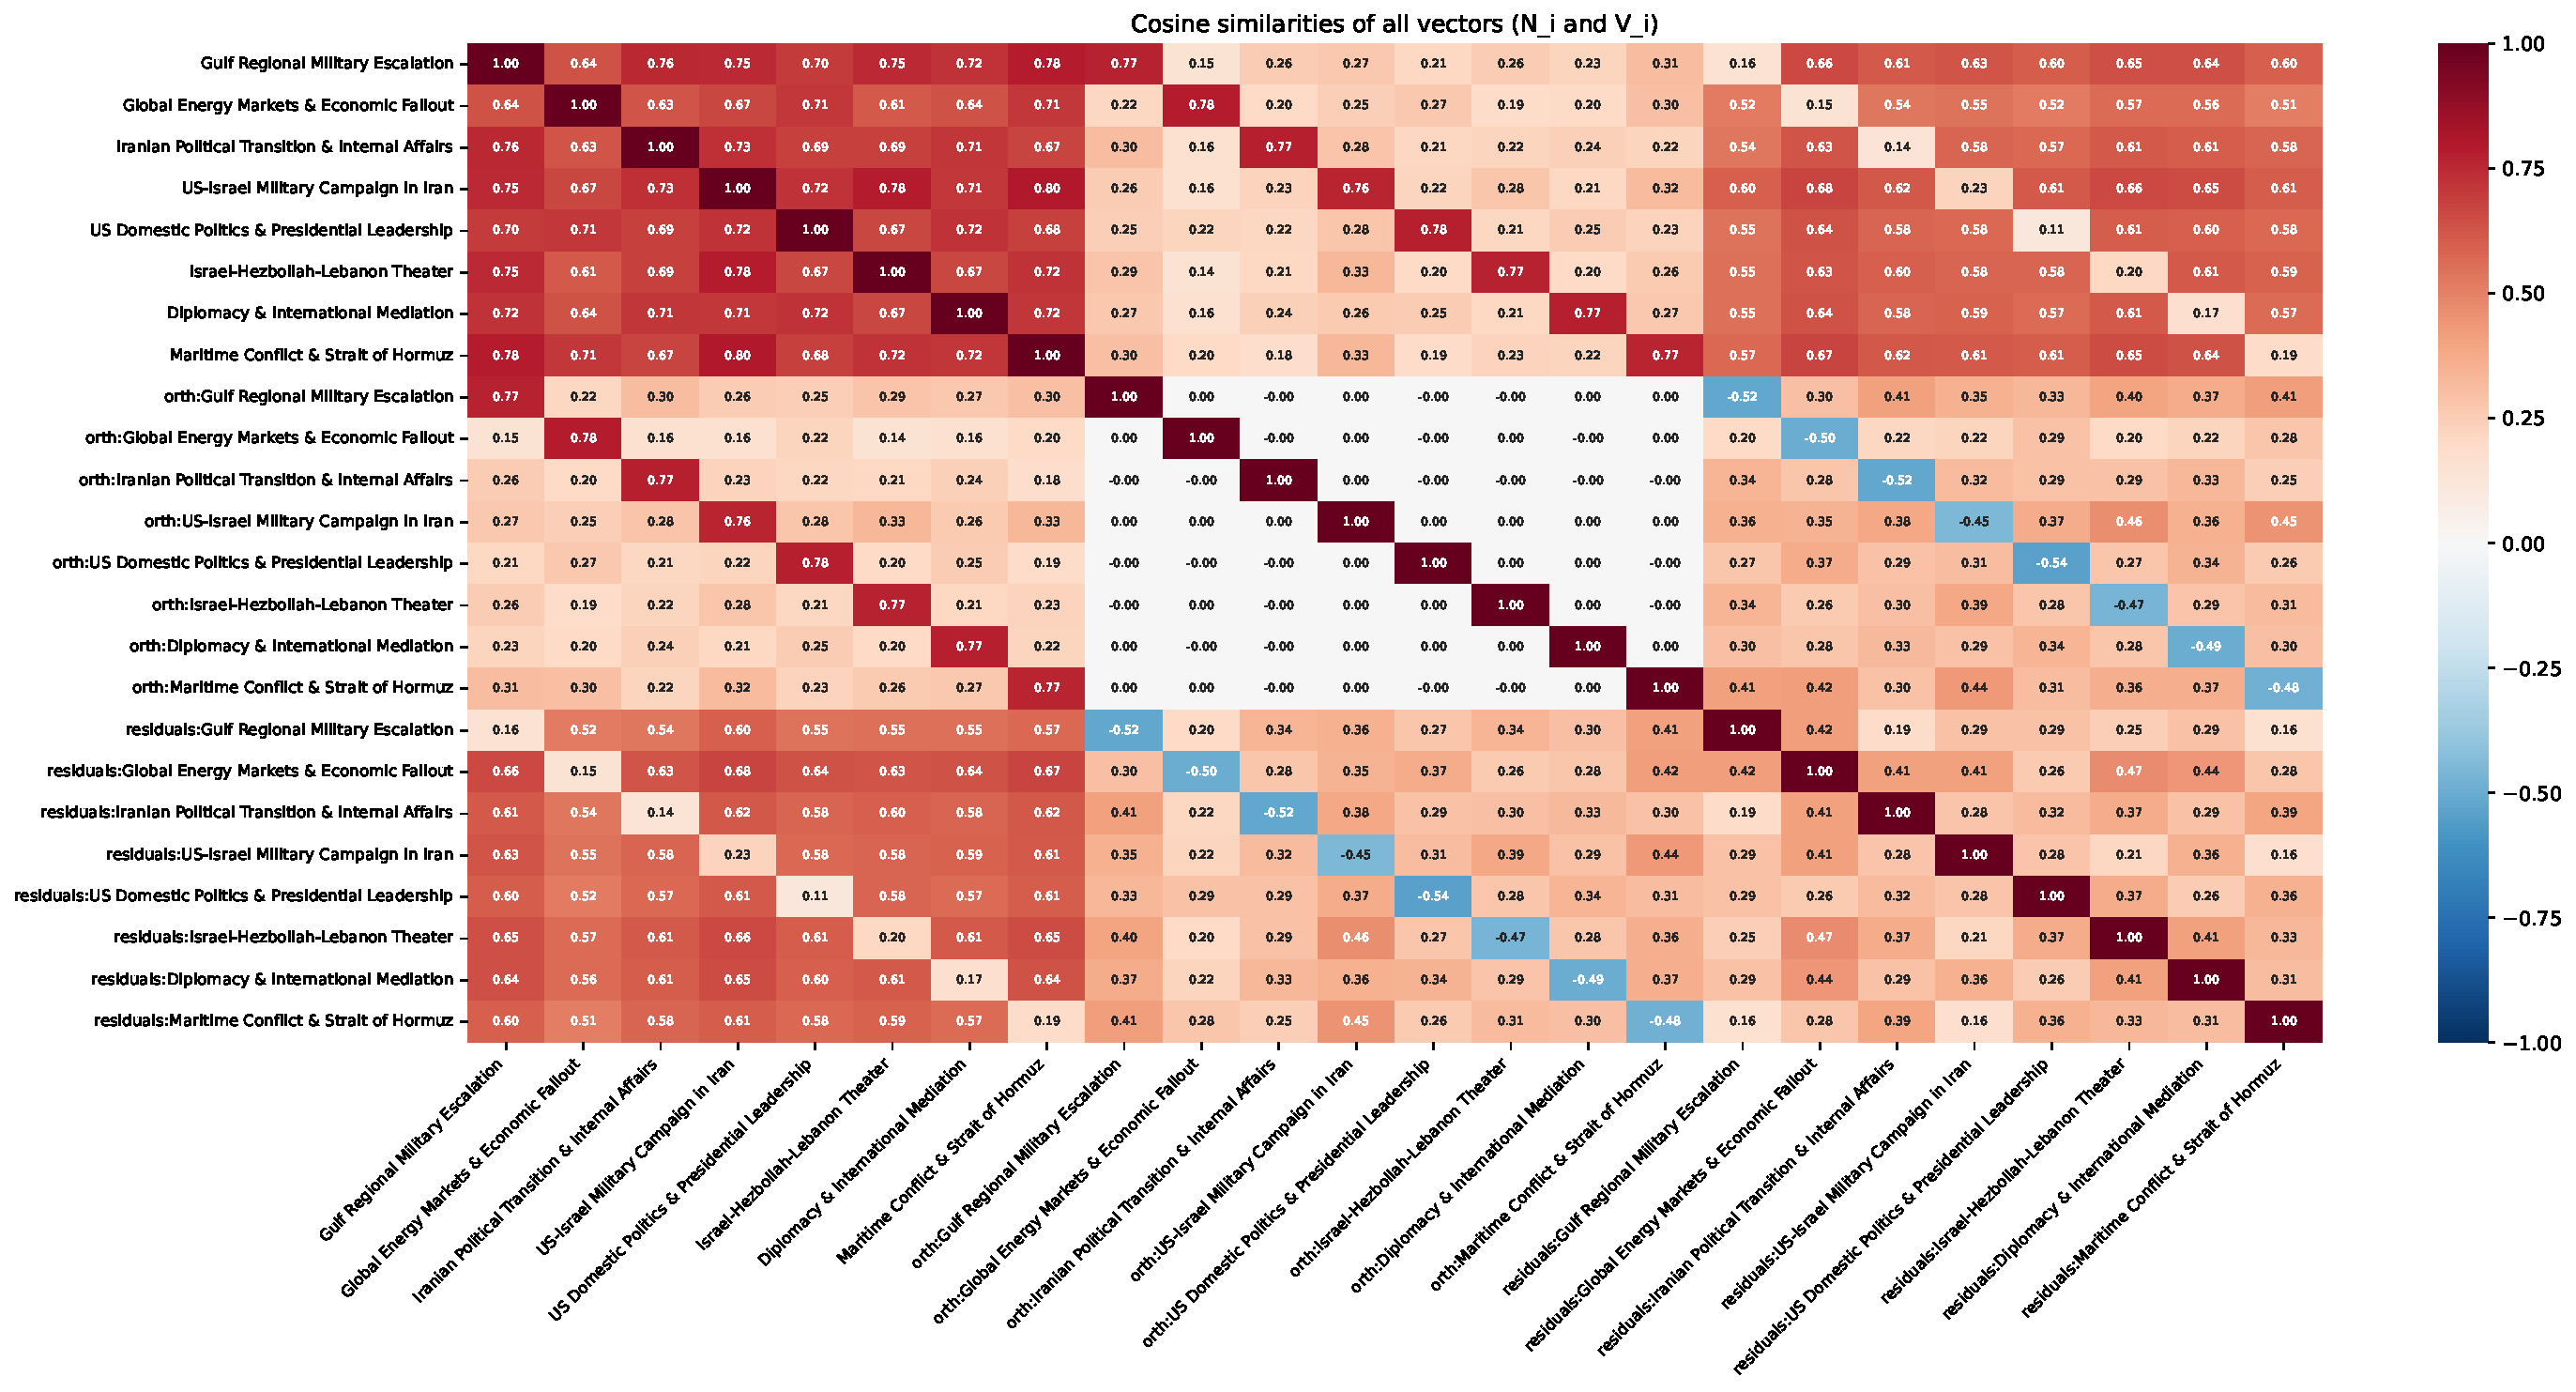
\includegraphics[width=0.95\textwidth]{cosine_similarities_avg.pdf}
\caption{Pairwise cosine similarity between the 8 original prototypes
(top-left block), the 8 orthogonalized prototypes (middle block, exactly
block-diagonal by construction), and the 8 residual vectors (bottom-right
block). Note how the original prototypes are highly inter-correlated
(0.6--0.8), whereas the orthogonal ones are, by construction, uncorrelated
with one another (off-diagonal $\approx 0$) yet remain well aligned with
their own original direction (values on the ``original vs.\ orth'' diagonal,
$\approx 0.7$--$0.8$).}
\label{fig:heatmap}
\end{figure}

% =========================================================================
\section{Stage 4: Scoring the corpus under three representations}
% =========================================================================

Every snippet $s_t$ ($t=1,\dots,1572$) already carries a K-Means cluster
label $c(t) \in \{1,\dots,8\}$ from Stage~1 --- a label obtained in the
\emph{natural embedding space}, before any orthogonalization existed.
Independently of that label, its embedding $\mathbf{e}_t$ is scored against
\emph{all eight} prototypes under each of the three representations
(prototype / pure narrative / residual), giving three $1572\times 8$
similarity matrices:
\[
S^{\text{orig}}_{t,i} = \mathbf{e}_t^\top \mathbf{N}_i, \qquad
S^{\text{orth}}_{t,i} = \mathbf{e}_t^\top \mathbf{V}_i, \qquad
S^{\text{res}}_{t,i} = \mathbf{e}_t^\top \mathbf{R}_i .
\]
Recall that $S^{\text{orth}}_{t,i}$ is, by the argument of
Section~\ref{sec:interpretation}, a measure of document $t$'s
\emph{relative exposure to the pure narrative of theme $i$}, cleaned of the
shared background noise that would otherwise contaminate
$S^{\text{orig}}_{t,i}$.
For each snippet, two quantities are then extracted for each representation:
\begin{itemize}
    \item \textbf{in-cluster similarity}: $S_{t,\,c(t)}$ --- similarity to the prototype of the snippet's own K-Means cluster;
    \item \textbf{out-of-cluster similarity}: $\{S_{t,j} : j \ne c(t)\}$ --- similarity to the seven other prototypes.
\end{itemize}

\begin{examplebox}{Worked example --- one snippet from \textit{Maritime Conflict}}
Consider the snippet (assigned by K-Means to \textit{Maritime Conflict \&
Strait of Hormuz}) reporting that only a handful of ships crossed the strait
on a given day because captains and owners remained cautious. Its similarity
profile is qualitatively:
\begin{center}
\begin{tabular}{lccc}
\toprule
Prototype ($j$) & $S^{\text{orig}}$ & $S^{\text{orth}}$ & $S^{\text{res}}$\\
\midrule
Maritime Conflict (own cluster, $j = c(t)$) & $\sim 0.80$ & $\sim 0.52$ & $\sim 0.30$\\
US-Israel Military Campaign & $\sim 0.75$ & $\sim 0.28$ & $\sim 0.55$\\
Diplomacy \& Mediation & $\sim 0.70$ & $\sim 0.22$ & $\sim 0.50$\\
\bottomrule
\end{tabular}
\end{center}
Under the \emph{original} representation, the snippet's own theme wins, but
only by a narrow margin over unrelated themes (0.80 vs.\ 0.70--0.75): the
raw embedding space is ``crowded''. Under the \emph{orthogonal}
representation, the margin widens sharply in relative terms (0.52 vs.\
0.22--0.28): once the shared conflict-reporting signal is projected out, the
snippet is unambiguously closest to its own, purified theme vector.
\end{examplebox}

% =========================================================================
\section{Stage 5: Ex post validation}
\label{sec:stage5}
% =========================================================================

If the K-Means clustering (Stage~1) and the prototype selection (Stage~2)
both captured a genuine underlying structure, we would expect the
\emph{orthogonalized} prototypes --- which were built completely
independently of the K-Means labels, from only 3 hand-picked sentences per
cluster --- to discriminate the 1{,}572 labelled documents \emph{better}
than the raw, correlated prototypes. This is exactly what is tested in
Figures~\ref{fig:boxplot} and~\ref{fig:barchart}.

\begin{figure}[htbp]
\centering
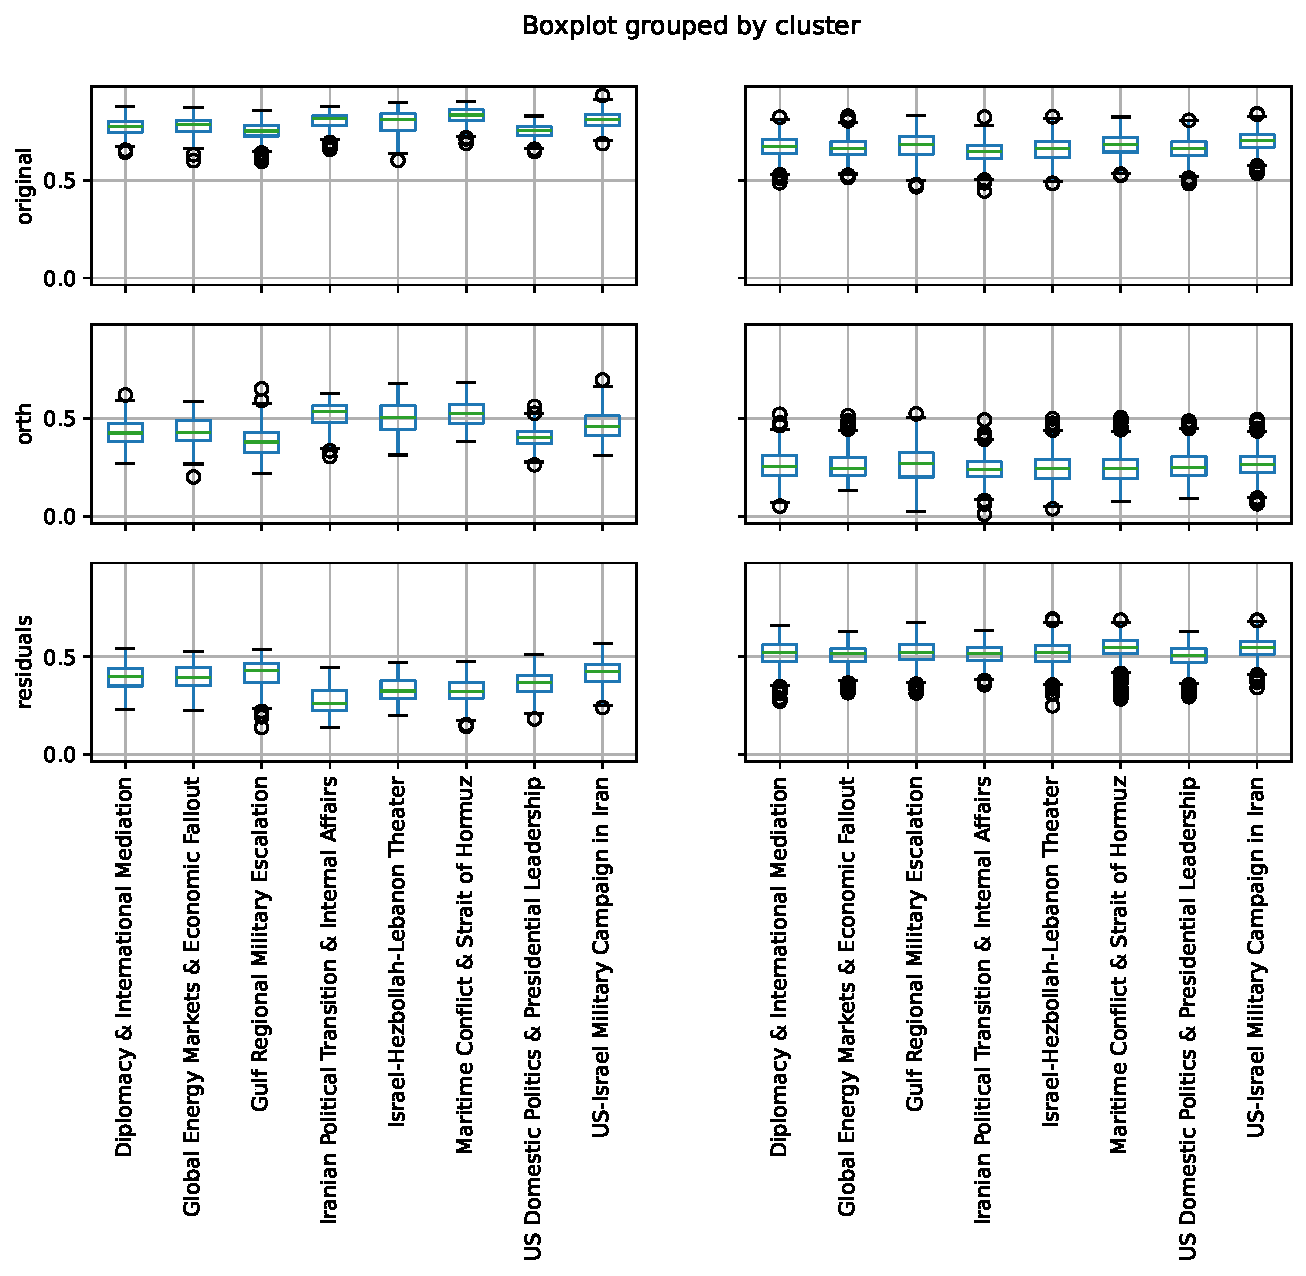
\includegraphics[width=0.98\textwidth]{compare_cosine_orth.pdf}
\caption{Distribution (boxplots) of cosine similarity scores, grouped by
theme, under the three representations (rows: original / orthogonal /
residual) and two conditions (columns: \emph{in-cluster} similarity --- a
document scored against the prototype of its own K-Means cluster; and
\emph{out-of-cluster} similarity --- the same document scored against the
other seven prototypes). Compare the vertical gap between the left and
right columns across rows: it is small for ``original'' and ``residuals'',
and comparatively much larger for ``orth''.}
\label{fig:boxplot}
\end{figure}

\begin{figure}[htbp]
\centering
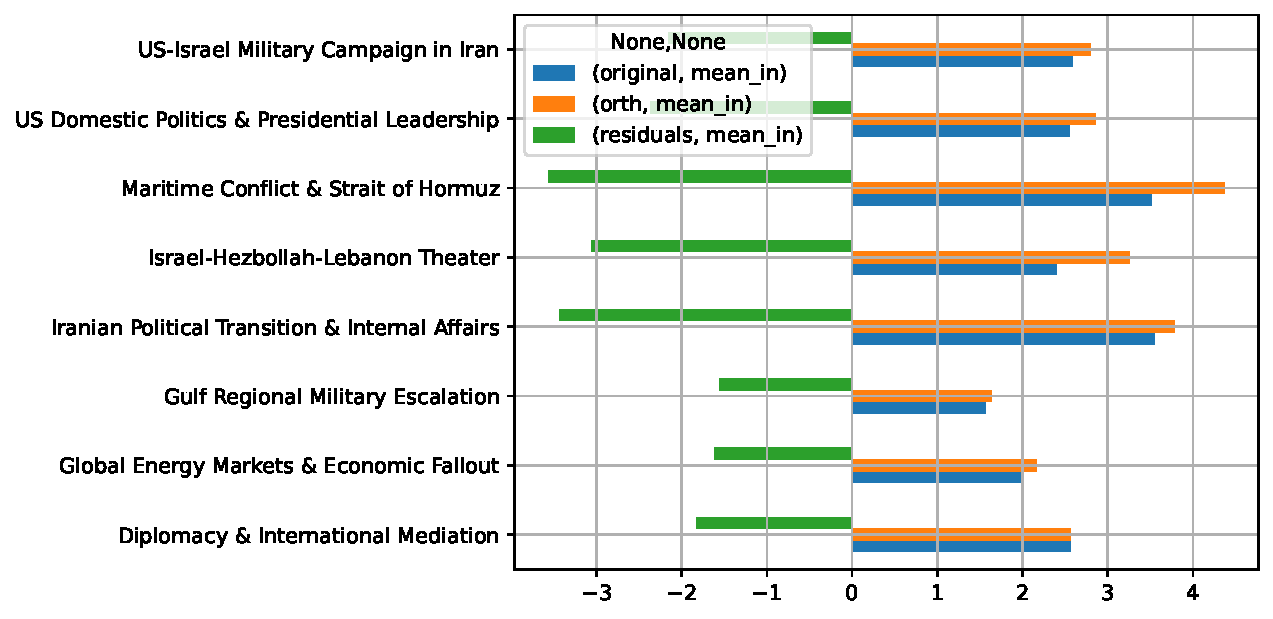
\includegraphics[width=0.85\textwidth]{compare_cosine_mean.pdf}
\caption{Standardized in-cluster separation, $(\overline{S}_{\text{in}} -
\overline{S}_{\text{out}})/\sigma_{\text{in}}$, for each theme and each
representation. Blue and orange bars (original vs.\ orthogonal) are of
comparable magnitude and consistently \emph{positive} for every theme,
confirming discriminative power in both representations; the orange
(orthogonal) bars are slightly larger than the blue (original) ones for
every single theme, indicating a systematic --- if moderate --- improvement
in separation once the shared component is projected out. Green bars
(residuals) are uniformly \emph{negative}: a document's similarity to the
\emph{residual} of its own cluster is, on average, \emph{lower} than to the
residuals of other clusters, which is the expected signature of a
component that carries generic, non-discriminative signal rather than
theme-specific signal.}
\label{fig:barchart}
\end{figure}

\begin{examplebox}{Worked example --- reading the result for \textit{Maritime Conflict}}
From Figure~\ref{fig:boxplot} (column ``Maritime Conflict \& Strait of
Hormuz''): under the \emph{original} representation, in-cluster similarity
(left column, top row) sits around 0.78--0.80 with essentially no overlap
with the out-of-cluster distribution (right column, top row, centered
$\approx 0.65$) --- already a reasonably clean separation, consistent with
this being one of the most lexically distinctive themes in the corpus
(shipping, tankers, blockades). Under the \emph{orthogonal} representation
(middle row), in-cluster similarity drops in absolute terms
($\approx 0.52$) but the out-of-cluster distribution drops \emph{much
further} ($\approx 0.27$), so that the standardized gap
(Fig.~\ref{fig:barchart}, ``Maritime Conflict'' row) is the \emph{largest of
all eight themes} ($\approx 4.3$ standard deviations, versus $\approx 3.5$
for the original representation). This is consistent with \textit{Maritime
Conflict} being a theme with a genuinely distinct technical vocabulary
(``Strait of Hormuz'', ``tanker'', ``blockade'') that survives the
orthogonalization essentially intact, while its correlation with other
themes (through shared war-reporting language) is precisely what gets
stripped out.
\end{examplebox}

\subsection{Take-away}
Across all eight themes (Fig.~\ref{fig:barchart}), the pure-narrative
(orthogonal) representation matches or exceeds the prototype's
discriminative power, while the residual (background-noise) representation
is uniformly non-discriminative (negative separation). Since the pure
narratives were derived from only three representative sentences per
cluster and an unsupervised geometric constraint (orthonormality),
\emph{not} from the K-Means labels themselves --- and since K-Means itself
was run on the untouched, natural embedding space (Section~2) --- this
constitutes an unsupervised, label-free corroboration that:
\begin{enumerate}
    \item the eight K-Means clusters correspond to genuinely separable narrative axes in the natural embedding space, and
    \item the Stiefel-manifold orthogonalization is not merely an algebraic transformation but recovers additional, meaningful discriminative signal --- the pure narrative --- that was masked by shared background noise in the raw prototypes, and
    \item consequently, tracking a document's (or a day's) similarity to a \emph{pure} narrative over time is a meaningful way to monitor exposure to that specific narrative, largely free of confounding drift in generic war-reporting language.
\end{enumerate}


\clearpage
\appendix
\section*{Appendix}

\section{Detailed cluster descriptions}
\label{app:clusters}

This appendix gives, for each of the eight K-Means clusters (natural
embedding space, Section~2), its thematic label, the rationale for that
label, and a short illustrative excerpt of the kind of reporting it
contains (paraphrased and abbreviated from the underlying CNN live-blog
text; original snippet indices are given in brackets for traceability).
Cluster sizes are repeated from Table~\ref{tab:clusters} for convenience.

\begin{description}[leftmargin=0pt, style=nextline, itemsep=8pt]

\item[Cluster 0 --- Gulf Regional Military Escalation ($n=209$)]
\textbf{Theme:} direct attacks, drone/missile interceptions, evacuations,
and security alerts across secondary Gulf states (Saudi Arabia, Kuwait, UAE,
Bahrain, Qatar, Iraq, Yemen). \textbf{Rationale:} distinct from the
Iran-centered strike cluster (Cluster 3), this group captures how hostilities
spread physically across the wider Gulf and Red Sea region, with an emphasis
on civilian infrastructure, air-defense activations, and evacuations of
foreign nationals. \textbf{Illustrative excerpts:} Saudi air defenses
intercepting drones near Riyadh \texttt{[2026-03-02 \#10]}; Qatar evacuating
residents near the US Embassy as a precaution \texttt{[2026-03-04 \#16]};
stranded travelers waiting out flight cancellations in Dhaka
\texttt{[2026-03-01 \#13]}.

\item[Cluster 1 --- Global Energy Markets \& Economic Fallout ($n=81$)]
\textbf{Theme:} oil-price surges, gas-price spikes, market volatility, and
government responses such as Strategic Petroleum Reserve releases.
\textbf{Rationale:} isolates financial/economic consequences of the war
(supply-chain and price effects) as distinct from the military actions that
cause them. \textbf{Illustrative excerpts:} Trump downplaying oil prices
above \$100/barrel \texttt{[2026-03-08 \#18]}; the SPR release of 172
million barrels \texttt{[2026-03-11 \#15]}; a small manufacturer describing
supply disruptions \texttt{[2026-03-21 \#10]}.

\item[Cluster 2 --- Iranian Political Transition \& Internal Affairs ($n=110$)]
\textbf{Theme:} Iran's internal governance, the death of Supreme Leader Ali
Khamenei, the succession of Mojtaba Khamenei, and domestic repression.
\textbf{Rationale:} groups reporting on internal regime dynamics that are
largely orthogonal, substantively, to the external military campaign.
\textbf{Illustrative excerpts:} the Assembly of Experts selecting a new
supreme leader \texttt{[2026-03-08 \#13]}; mass mourning crowds during the
multi-day funeral \texttt{[2026-07-06 \#5]}; reports of a wave of political
executions \texttt{[2026-05-06 \#4]}.

\item[Cluster 3 --- US-Israel Military Campaign in Iran ($n=246$)]
\textbf{Theme:} direct kinetic operations --- airstrikes, missile exchanges,
naval engagements --- between US/Israeli forces and Iranian military
targets, including CENTCOM operational updates. \textbf{Rationale:}
this is the ``main campaign'' cluster, defined by strike counts, named
targets (e.g.\ Kharg Island), and official military communiqu\'es.
\textbf{Illustrative excerpts:} over 3,000 targets struck under Operation
``Epic Fury'' \texttt{[2026-03-06 \#8]}; strikes on Kharg Island oil
infrastructure \texttt{[2026-03-13 \#4]}; CENTCOM footage of naval strikes
near Hormuz \texttt{[2026-03-10 \#16]}.

\item[Cluster 4 --- US Domestic Politics \& Presidential Leadership ($n=306$)]
\textbf{Theme:} White House rhetoric, presidential statements, press
briefings, and congressional oversight debates. \textbf{Rationale:} this
cluster is anchored in Washington politics --- how the US executive
communicates and defends its war strategy domestically --- rather than in
events on the ground. \textbf{Illustrative excerpts:} Trump outlining war
objectives to reporters \texttt{[2026-03-02 \#0]}; a White House press
briefing on administration resolve \texttt{[2026-03-25 \#13]}; Senate
Democrats forcing a war-powers vote \texttt{[2026-03-09 \#12]}.

\item[Cluster 5 --- Israel-Hezbollah-Lebanon Theater ($n=170$)]
\textbf{Theme:} the parallel Israel--Hezbollah/Lebanon (and adjacent Gaza)
front: rocket and airstrike exchanges, ground movements, and fragile
ceasefires. \textbf{Rationale:} separates the Mediterranean flank of the
conflict from the Iran-centered campaign (Cluster 3), since the actors,
geography, and ceasefire dynamics differ substantially.
\textbf{Illustrative excerpts:} Israel intensifying strikes on Lebanon
\texttt{[2026-03-01 \#7]}; Hezbollah rocket fire damaging homes in central
Israel \texttt{[2026-03-12 \#18]}; a fragile Lebanon-Israel ceasefire under
strain \texttt{[2026-06-04 \#10]}.

\item[Cluster 6 --- Diplomacy \& International Mediation ($n=235$)]
\textbf{Theme:} diplomatic backchannels, mediated negotiations (chiefly by
Qatar, Pakistan, and Oman), and the drafting of ceasefire or peace
frameworks. \textbf{Rationale:} isolates official diplomatic statements and
mediation efforts, as distinct from the military and domestic-political
narratives. \textbf{Illustrative excerpts:} Pakistan offering to host
US-Iran talks \texttt{[2026-03-23 \#12]}; envoys Witkoff and Kushner meeting
Qatar's prime minister \texttt{[2026-06-30 \#1]}; a trilateral defense pact
among Saudi Arabia, Turkey, and Pakistan \texttt{[2026-08-07 \#1]}.

\item[Cluster 7 --- Maritime Conflict \& Strait of Hormuz ($n=215$)]
\textbf{Theme:} commercial shipping disruption, naval blockades, tanker
attacks, and transit management in the Strait of Hormuz and the wider
Persian Gulf. \textbf{Rationale:} a domain-specific cluster with a
distinctive technical vocabulary (tankers, chokepoints, transit risk),
used as the worked example throughout the main text.
\textbf{Illustrative excerpts:} traffic through the Strait crawling to a
near halt \texttt{[2026-03-03 \#18]}; a container vessel damaged off the
UAE coast \texttt{[2026-03-10 \#2]}; US Marines seizing an Iranian-flagged
cargo ship attempting to run the blockade \texttt{[2026-04-20 \#5]}.

\end{description}

\end{document}
